
%%\documentclass[12pt,preprint]{aastex}

%% manuscript produces a one-column, double-spaced document:

%% \documentclass[10pt,manuscript]{aastex}

%% preprint2 produces a double-column, single-spaced document:
\documentclass[preprint2,apjl,numberedappendix,twocolappendix,appendixfloats]{emulateapj}
%% \documentclass[preprint2,iop]{aastex}

%% \documentclass[preprint2,longabstract]{aastex}

%% \usepackage{ccaption}
%% \captionstyle{\raggedright}
\usepackage[caption=false]{subfig}
\usepackage{amsmath}
\usepackage{footnote}
\bibpunct{(}{)}{;}{a}{}{,} 
\captionsetup{belowskip=12pt,aboveskip=4pt}
\setlength{\textfloatsep}{10pt plus 1.0pt minus 2.0pt}
\newcommand{\dif}{\mathrm{d}}
%% \renewcommand*{\thefootnote}{\fnsymbol{footnote}}

\def\nar{{New~A~Rev.}}          % New Astronomy Review
\def\pasa{{PASA}}               % Publications of the Astron. Soc. of Australia

%% \bibliographystyle{mn2e}
%% \bibliographystyle{apj}

\shorttitle{Wide--field Effects in EoR Power Spectra}
\shortauthors{Thyagarajan et~al.}

\def\ASU{\altaffilmark{1}}
\def\ASUtxt{\altaffiltext{1}{Arizona State University, School of Earth and Space Exploration, Tempe, AZ 85287, USA}}

\def\myemail{\altaffilmark{*}}
\def\myemailtxt{\altaffiltext{*}{e-mail: t\_nithyanandan@asu.edu}}

\def\UW{\altaffilmark{2}}
\def\UWtxt{\altaffiltext{2}{University of Washington, Department of Physics, Seattle, WA 98195, USA}}

\def\SKASA{\altaffilmark{3}}
\def\SKASAtxt{\altaffiltext{3}{Square Kilometre Array South Africa (SKA SA), Park Road, Pinelands 7405, South Africa}}

\def\RU{\altaffilmark{4}}
\def\RUtxt{\altaffiltext{4}{Department of Physics and Electronics, Rhodes University, Grahamstown 6140, South Africa}}

\def\CfA{\altaffilmark{5}}
\def\CfAtxt{\altaffiltext{5}{Harvard-Smithsonian Center for Astrophysics, Cambridge, MA 02138, USA}}

\def\ANU{\altaffilmark{6}}
\def\ANUtxt{\altaffiltext{6}{Australian National University, Research School of Astronomy and Astrophysics, Canberra, ACT 2611, Australia}}

\def\CAASTRO{\altaffilmark{7}}
\def\CAASTROtxt{\altaffiltext{7}{ARC Centre of Excellence for All-sky Astrophysics (CAASTRO)}}

\def\Haystack{\altaffilmark{8}}
\def\Haystacktxt{\altaffiltext{8}{MIT Haystack Observatory, Westford, MA 01886, USA}}

\def\MIT{\altaffilmark{9}}
\def\MITtxt{\altaffiltext{9}{MIT Kavli Institute for Astrophysics and Space Research, Cambridge, MA 02139, USA}}

\def\Curtin{\altaffilmark{10}}
\def\Curtintxt{\altaffiltext{10}{International Centre for Radio Astronomy Research, Curtin University, Perth, WA 6845, Australia}}

\def\Victoria{\altaffilmark{11}}
\def\Victoriatxt{\altaffiltext{11}{Victoria University of Wellington, School of Chemical \& Physical Sciences, Wellington 6140, New Zealand}}

\def\UWisc{\altaffilmark{12}}
\def\UWisctxt{\altaffiltext{12}{University of Wisconsin--Milwaukee, Department of Physics, Milwaukee, WI 53201, USA}}

\def\UMichigan{\altaffilmark{13}}
\def\UMichigantxt{\altaffiltext{13}{University of Michigan, Department of Atmospheric, Oceanic and Space Sciences, Ann Arbor, MI 48109, USA}}

\def\UMelbourne{\altaffilmark{14}}
\def\UMelbournetxt{\altaffiltext{14}{The University of Melbourne, School of Physics, Parkville, VIC 3010, Australia}}

\def\USydney{\altaffilmark{15}}
\def\USydneytxt{\altaffiltext{15}{The University of Sydney, Sydney Institute for Astronomy, School of Physics, NSW 2006, Australia}}

\def\CASS{\altaffilmark{16}}
\def\CASStxt{\altaffiltext{16}{CSIRO Astronomy and Space Science (CASS), PO Box 76, Epping, NSW 1710, Australia}}

\def\Tata{\altaffilmark{17}}
\def\Tatatxt{\altaffiltext{17}{National Centre for Radio Astrophysics, Tata Institute for Fundamental Research, Pune 411007, India}}

\def\RRI{\altaffilmark{18}}
\def\RRItxt{\altaffiltext{18}{Raman Research Institute, Bangalore 560080, India}}

\def\NRAO{\altaffilmark{19}}
\def\NRAOtxt{\altaffiltext{19}{National Radio Astronomy Observatory, Charlottesville and Greenbank, USA}}

\def\UWA{\altaffilmark{20}}
\def\UWAtxt{\altaffiltext{20}{International Centre for Radio Astronomy Research, University of Western Australia, Crawley, WA 6009, Australia}}

%% \definenote[thanks][conversion=set 2]

\begin{document}

\title{Wide--Field Effects in Redshifted 21~cm Power Spectra}

%% Use \author, \affil, and the \and command to format
%% author and affiliation information.
%% Note that \email has replaced the old \authoremail command
%% from AASTeX v4.0. You can use \email to mark an email address
%% anywhere in the paper, not just in the front matter.
%% As in the title, use \\ to force line breaks.

%% Author list
\author{
%% Lead Authors
Nithyanandan~Thyagarajan\ASU\myemail,
Daniel~C.~Jacobs\ASU,
Judd~D.~Bowman\ASU,
N.~Barry\UW,
A.~P.~Beardsley\UW,
G.~Bernardi\SKASA$^,$\RU$^,$\CfA,
F.~Briggs\ANU$^,$\CAASTRO,
R.~J.~Cappallo\Haystack, 
P.~Carroll\UW,
B.~E.~Corey\Haystack, 
% A.~A.~Deshpande\RRI, 
A.~de~Oliveira-Costa\MIT,
Joshua~S.~Dillon\MIT,
D.~Emrich\Curtin,
% B.~M.~Gaensler\USydney$^,$\CAASTRO, 
A.~Ewall-Wice\MIT,
L.~Feng\MIT,
R.~Goeke\MIT,
L.~J.~Greenhill\CfA,
B.~J.~Hazelton\UW, 
J.~N.~Hewitt\MIT,
N.~Hurley-Walker\Curtin,
M.~Johnston-Hollitt\Victoria,
D.~L.~Kaplan\UWisc, 
J.~C.~Kasper\UMichigan$^,$\CfA, 
Han-Seek Kim\UMelbourne$^,$\CAASTRO,
P.~Kittiwisit\ASU,
E.~Kratzenberg\Haystack, 
E.~Lenc\USydney$^,$\CAASTRO,
J.~Line\UMelbourne$^,$\CAASTRO,
A.~Loeb\CfA,
C.~J.~Lonsdale\Haystack, 
M.~J.~Lynch\Curtin, 
B.~McKinley\UMelbourne$^,$\CAASTRO,
S.~R.~McWhirter\Haystack,
D.~A.~Mitchell\CASS$^,$\CAASTRO, 
M.~F.~Morales\UW, 
E.~Morgan\MIT, 
A.~R.~Neben\MIT,
D.~Oberoi\Tata, 
A.~R.~Offringa\ANU$^,$\CAASTRO, 
S.~M.~Ord\Curtin$^,$\CAASTRO,
Sourabh~Paul\RRI,
B.~Pindor\UMelbourne$^,$\CAASTRO,
J.~C.~Pober\UW,
T.~Prabu\RRI, 
P.~Procopio\UMelbourne$^,$\CAASTRO,
J.~Riding\UMelbourne$^,$\CAASTRO,
A.~E.~E.~Rogers\Haystack, 
A.~Roshi\NRAO, 
N.~Udaya~Shankar\RRI, 
Shiv~K.~Sethi\RRI,
K.~S.~Srivani\RRI, 
R.~Subrahmanyan\RRI$^,$\CAASTRO, 
I.~S.~Sullivan\UW,
M.~Tegmark\MIT,
S.~J.~Tingay\Curtin$^,$\CAASTRO, 
C.~M.~Trott\Curtin$^,$\CAASTRO,
M.~Waterson\Curtin$^,$\ANU,
R.~B.~Wayth\Curtin$^,$\CAASTRO, 
R.~L.~Webster\UMelbourne$^,$\CAASTRO, 
A.~R.~Whitney\Haystack, 
A.~Williams\Curtin, 
C.~L.~Williams\MIT,
C.~Wu\UWA,
J.~S.~B.~Wyithe\UMelbourne$^,$\CAASTRO
}

%Institutional footnotes (typeset, then rearrange here to be in order)
\ASUtxt
\UWtxt
\SKASAtxt
\RUtxt
\CfAtxt
\ANUtxt
\CAASTROtxt
\Haystacktxt
\MITtxt
\Curtintxt
\Victoriatxt
\UWisctxt
\UMichigantxt
\UMelbournetxt
\USydneytxt
\CASStxt
\Tatatxt
\RRItxt
\NRAOtxt
\UWAtxt
\myemailtxt

%% \email{t\_nithyanandan@rri.res.in}

%% \clearpage

\begin{abstract}

Foreground emission is currently the primary limitation to detection of redshifted H{\sc i} emission from the epoch of reionization. Modern radio telescopes that target this cosmological signal are typically wide--field instruments. Through modeling of delay spectra measured between antenna pairs, it has recently emerged that wide--field measurements imprint a characteristic {\it pitchfork}--shaped signature in this Fourier domain. This predicted feature is characterized by enhanced power from foreground emission mapped to regions near the horizon and plays a significant role in determining the contamination of the cosmological H{\sc i} signal. With MWA data sensitivity improved by coherently averaging 12 independent snapshots aligned in local sidereal time across different observing nights, we confirm the prediction with a signal--noise ratio $>10$.

\end{abstract}
 
\keywords{cosmology: observations --- dark ages, reionization, first stars --- large-scale structure of universe --- methods: statistical --- radio continuum: galaxies --- techniques: interferometric}

\section{Introduction}\label{sec:intro}



\section{Wide--Field Effects in Delay Spectrum}\label{sec:wide-field}

\citet{thy15} have described in detail the effects of wide--field measurements as seen in the delay spectra of interferometer {\it visibilities}. Here, we give a brief overview of the wide--field signature predicted therein. 

The delay spectrum for a baseline vector, $\boldsymbol{b}$, is given by \citep{par12a,par12b,thy13,thy15}: 
\begin{align}
  \tilde{V}_b(\tau) &\equiv \int V_b(f)\,W(f)\,e^{i2\pi f\tau}\,\dif f,
\end{align}
with interferometer visibilities, $V_b(f)$, given by \citep{van34,zer38,tho01}:
\begin{align} 
  V_b(f) &= \iint\limits_\textrm{sky} A(\hat{\boldsymbol{s}},f)\,I(\hat{\boldsymbol{s}},f)\,W_\textrm{i}(f)\,e^{-i2\pi f\frac{\boldsymbol{b}\cdot\hat{\boldsymbol{s}}}{c}}\,\dif\Omega \\
         &= \iint\limits_\textrm{sky} \frac{A(\hat{\boldsymbol{s}},f)\,I(\hat{\boldsymbol{s}},f)}{\sqrt{1-l^2-m^2}}\,W_\textrm{i}(f)\,e^{-i2\pi f\frac{\boldsymbol{b}\cdot\hat{\boldsymbol{s}}}{c}}\,\dif l\,\dif m, 
\end{align}
where, $I(\hat{\boldsymbol{s}},f)$ and $A(\hat{\boldsymbol{s}},f)$ are the sky brightness and antenna's directional power pattern, respectively, as a function of frequency ($f$) and direction on the sky denoted by the unit vector $\hat{\boldsymbol{s}}\equiv (l,m,n)$, $W_\textrm{i}(f)$ denotes instrumental bandpass weights, $W(f)$ is a spectral weighting function that controls the transfer function in the delay transform, $\dif\Omega=(1-l^2-m^2)^{-1/2}\,\dif l\,\dif m$ is the solid angle element to which $\hat{\boldsymbol{s}}$ is the unit normal vector, and $c$ is the speed of light. $\tau=\boldsymbol{b}\cdot\hat{\boldsymbol{s}}/c$ is the geometric delay between antenna pairs measured relative to the zenith and provides a mapping to position on the sky.

In wide--field measurements, the steep rise in subtended solid angle near the horizon for a fixed delay bin size significantly enhances the integrated emission near the horizon delay limits. This is found to be true for diffuse emission even on wide antenna spacings because their foreshortening towards the horizon makes them sensitive to large angular scales that match the inverse of their foreshortened lengths. 

Typically, an antenna is most sensitive towards its primary field of view relative to the rest of the sky, which in conjunction with the aforementioned wide--field effects results in a characteristic ``pitchfork'' signature in the delay spectrum. 

Although there is marginal evidence for presence of this feature in the {\it zenith} snapshot presented in \citet{thy15}, the high level of thermal noise prevented a robust confirmation. In this paper, we confirm the {\it pitchfork} signature using deeper data from the MWA.

\section{The Murchison Widefield Array Observations}\label{sec:MWA}

The MWA instrument configuration, EoR observations, and data analysis used in this study are already described in \citet{thy15}. In order to reduce thermal fluctuations while maintaining coherence, it is essential to average independent data sets obtained over the same region of sky with identical beamformer settings. Hence, we select a subset of MWA snapshots each of duration 112~seconds obtained over different nights which are aligned to within 72~seconds of each other in {\it local sidereal time} (LST) around a mean LST of 0.04~hours with the MWA tile beam pointed at zenith. The database contains 14 snapshots satisfying these criteria. Two of these snapshots were found to contain amplitude and phase artifacts for a significant duration across different baselines. Hence, they have been excluded from our analysis. 

The delay spectra of the rest of the snapshots were verified to be coherent in their amplitudes and phases. These complex valued delay spectra from independent snapshots are averaged together to lower thermal fluctuations without losing coherence from foreground contributions. The results are discussed below.

\section{Results}\label{sec:results}

Figure~\ref{fig:avg-fhd-delay-spectra} shows the delay spectra obtained by averaging LST aligned delay spectra from individual snapshots from different nights. The dynamic range (in power spectrum units) in the averaged data is $\gtrsim 10$ higher compared to that in the {\it zenith} snapshot used in \citet{thy15}, and is consistent with the improvement expected in averaging 12 independent snapshots. With this improvement in sensitivity, the foreground power near the horizon limits (white dotted lines) has become $\gtrsim 10$ times more prominent. We also note that faint horizontal features appear at $\tau = \pm 0.78\,\mu$s also as a result of lowering thermal fluctuations which were not seen earlier in the individual snapshots presented in \citet{thy15}, thus confirming effective lowering of thermal fluctuations. We identify these faint features as the response in delay space of the MWA coarse band edges flagged periodically every 1.28~MHz. 

\begin{figure}[htb]
\centering
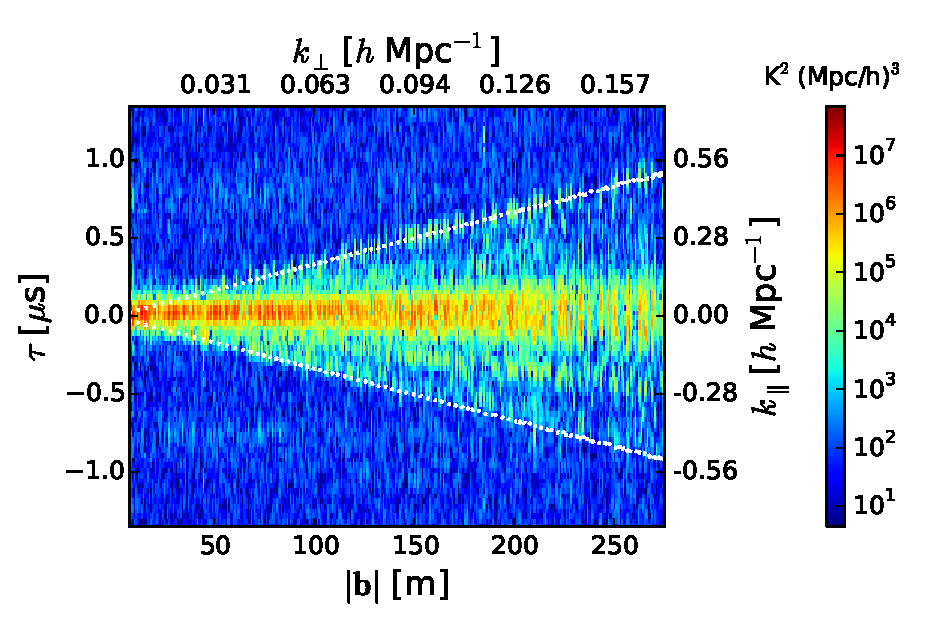
\includegraphics[width=\linewidth]{multi_baseline_CLEAN_fhd_avg_visibilities_amplitudes_185.0_MHz_30.7_MHz.eps}
\caption{Amplitudes of delay power spectra obtained by averaging 12 snapshots of LST aligned MWA data. The $x$--axis, denoted by $|\boldsymbol{b}|$ (and $k_\perp$), represents angular (and spatial) scales in the plane of the sky while the $y$--axis, shown in $\tau$ and $k_\parallel$, denotes the spatial scales along the line of sight. White dotted lines are the horizon delay limits. Power near the horizon limits caused by wide--field effects are prominent. Faint horizontal features at $\tau=\pm 0.78\,\mu$s are visible due to effective lowering of thermal fluctuations and are the response to periodic coarse band edge flagging of MWA data every 1.28~MHz. \label{fig:avg-fhd-delay-spectra}}
\end{figure}

Figure~\ref{fig:3-baseline-comparison-delay-spectra} shows the amplitudes of averaged delay spectra on three selected baseline vectors oriented northward. Data and noiseless simulations (using foreground and instrument models described in \citet{thy15}) are shown in black and red respectively. The horizontal dotted black line denotes {\it rms} of thermal fluctuations estimated from data. The vertical dashed line denotes horizon delay limits, and the vertical dot--dashed lines denote delays at which the responses to coarse band edge flagging are expected.

\begin{figure}[htb]
\centering
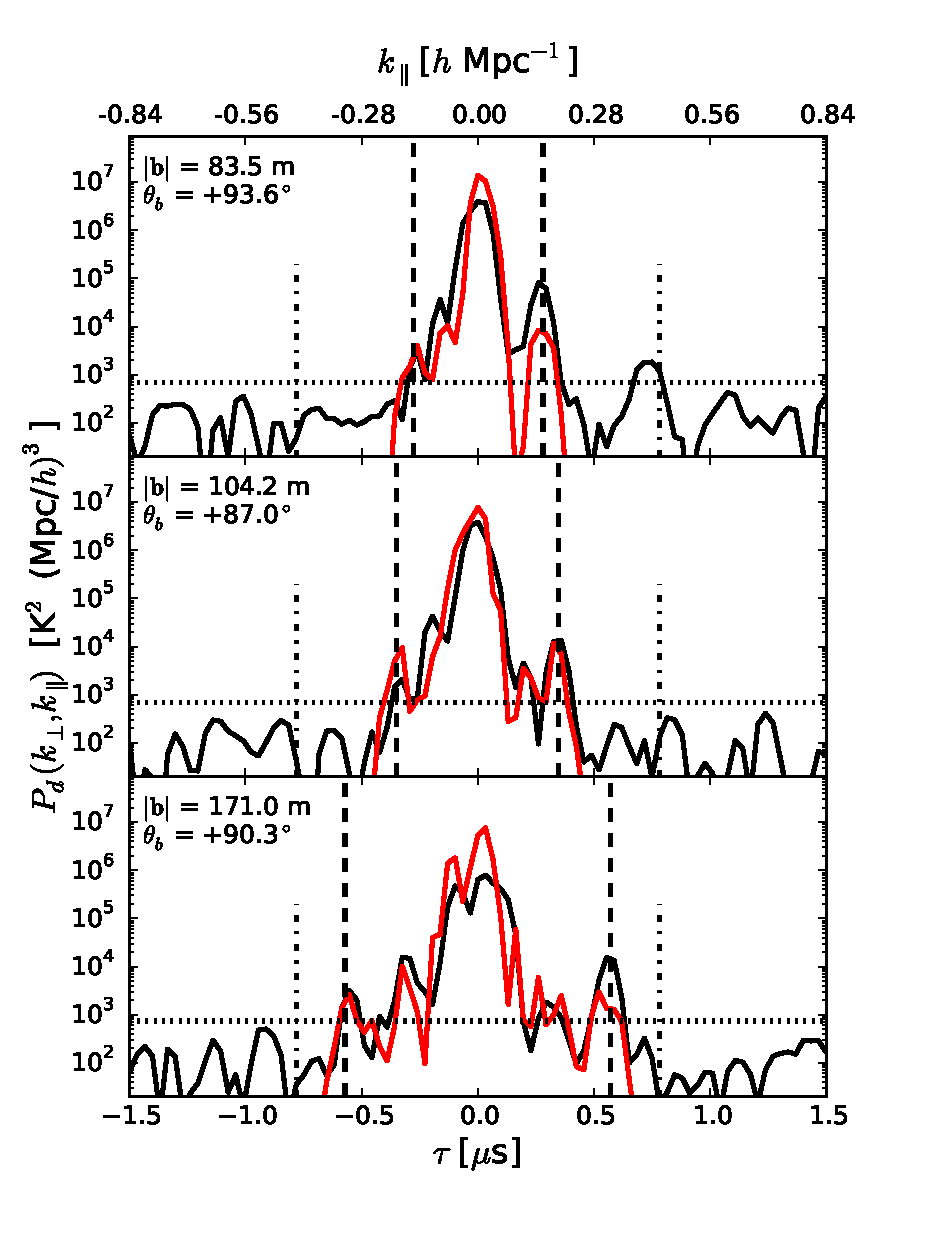
\includegraphics[width=\linewidth]{3_baseline_comparison_CLEAN_fhd_avg_visibilities_amplitudes_185.0_MHz_30.7_MHz.eps}
\caption{Delay power spectra amplitudes on three antenna spacings oriented northward obtained by coherent averaging of 12 snapshots aligned in LST. The data and models are shown in black and red respectively. The antenna spacings are 83.5~m ({\it top}), 104.2~m ({\it middle}), and 171~m ({\it bottom}). The horizontal dotted line is the {\it rms} of thermal fluctuations. The vertical dashed lines denote the horizon delay limits. The vertical dot--dashed lines at $\tau=\pm 0.78\,\mu$s correspond to grating responses of periodic flagging of bandpass at intervals of 1.28~MHz. The dynamic range has increased by a factor $\sim 10$ as a result of coherent averaging relative to that in \citet{thy15}. The peaks close to the horizon delay limits are distinctly visible at $\sim 10$--1000~$\sigma$ levels. Differences between model and data are primarily attributed to uncertainties in the foreground model and the MWA tile power pattern. \label{fig:3-baseline-comparison-delay-spectra}}
\end{figure}

The delay power spectra morphologies from data and modeling are remarkably similar even while ignoring any differences in the amplitude scales. We attribute these differences to uncertainties in the foreground model, the MWA tile power pattern, thermal fluctuations, and other uncertainties noted in \citet{thy15}. 

We focus on the level of foreground power near the horizon limits in the data. Typically, the power near the negative horizon limit is seen with a signal--noise ratio (SNR) $\sim$~10--100, while that around the positive horizon limit is $\sim$~100--1000. The models of \citet{thy15} have noted that the foreground power near the horizon limits is due to the nature of wide--field measurements, and is predominantly composed of diffuse emission especially on baseline lengths $\lesssim 100$~m. Based on the morphological agreement between the data and the models, we conclude the features noted in our current analysis are a robust detection of the {\it pitchfork} signature predicted in \citet{thy15}.

\section{Summary}\label{sec:summary}

Fluctuations of redshifted H{\sc i} from the reionization epoch are extremely faint relative to the radio continuum emission from foreground objects. This poses perhaps the greatest challenge to EoR experiments and therefore merits a detailed characterization of foreground signatures in order to separate them from the desired signal. 

In a recent study, through the use of models for an all--sky foreground and the instrument, the role of wide--field nature of modern radio interferometric measurements, hitherto unpredicted, has emerged. It is referred to as the {\it pitchfork} signature in the delay spectral domain, and is characterized by significant foreground power in the primary field of view and an enhancement in power near the horizon. The latter is due to the highly non--linear mapping between geometric delays and subtended solid angles besides an increase in sensitivity to larger scales caused by foreshortening of baseline lengths along these directions. This feature could not be confirmed in individual MWA snapshot observations due to the high level of thermal fluctuations. 

By averaging 12 independent snapshots tightly aligned in LST from MWA observations, we improve the dynamic range in delay power spectra by a factor $\gtrsim$~10 while maintaining the coherency of the observed {\it visibilities}. Foreground power in delay bins near the horizon is distinctly visible with a signal--noise ratio $>10$. In addition, there is a close resemblance in the morphologies of delay power spectra from data and models. Together, they allow us to make a robust confirmation of the nature of wide--field measurements in EoR experiments.

\acknowledgments

This work was supported by the U. S. National Science Foundation (NSF) through award AST--1109257. DCJ is supported by an NSF Astronomy and Astrophysics Postdoctoral Fellowship under award AST--1401708. JCP is supported by an NSF Astronomy and Astrophysics Fellowship under award AST-1302774. This work makes use of the Murchison Radio-astronomy Observatory, operated by CSIRO. We acknowledge the Wajarri Yamatji people as the traditional owners of the Observatory site. Support for the MWA comes from the NSF (awards: AST-0457585, PHY-0835713, CAREER-0847753, and AST-0908884), the Australian Research Council (LIEF grants LE0775621 and LE0882938), the U.S. Air Force Office of Scientific Research (grant FA9550-0510247), and the Centre for All-sky Astrophysics (an Australian Research Council Centre of Excellence funded by grant CE110001020). Support is also provided by the Smithsonian Astrophysical Observatory, the MIT School of Science, the Raman Research Institute, the Australian National University, and the Victoria University of Wellington (via grant MED-E1799 from the New Zealand Ministry of Economic Development and an IBM Shared University Research Grant). The Australian Federal government provides additional support via the Commonwealth Scientific and Industrial Research Organisation (CSIRO), National Collaborative Research Infrastructure Strategy, Education Investment Fund, and the Australia India Strategic Research Fund, and Astronomy Australia Limited, under contract to Curtin University. We acknowledge the iVEC Petabyte Data Store, the Initiative in Innovative Computing and the CUDA Center for Excellence sponsored by NVIDIA at Harvard University, and the International Centre for Radio Astronomy Research (ICRAR), a Joint Venture of Curtin University and The University of Western Australia, funded by the Western Australian State government.  

% \par\bigskip
\bibliographystyle{apj}
\bibliography{eor}

\end{document}
